\chapter{ \MakeUppercase{ SYSTEM METHODOLOGY}}\label{ch: method}


This chapter describes the methodology of the Integrated Document Verification Platform. It traces the full verification workflow from the initial document upload and text extraction, through the three stage XAI analysis, to the final anchoring of results on the Ethereum blockchain. For each stage, the underlying technique is explained along with the design rationale.

\section{Overall System Architecture}
\label{sec:system_architecture}
    The framework is built on a Modular Hybrid Architecture, meaning it divides responsibilities among four specialized layers that communicate through well-defined interfaces. Each layer operates independently and can be updated or replaced without affecting the others. The four layers and their responsibilities are summarized in Table 3.1.

    \begin{table}[htbp]
        \centering
        \caption{System Architecture Layers}
        \label{tab:system_architecture_layers}
        \renewcommand{\arraystretch}{1.4}
        
        \begin{tabular}{|p{3.5cm}|p{7cm}|p{4.5cm}|}
        \hline
        \textbf{Layer} & \textbf{Primary Responsibility} & \textbf{Key Technologies} \\
        \hline
        
        Web System (Frontend + Backend) &
        Request handling, file upload management, routing, and workflow coordination &
        Node.js, Express.js, Multer \\
        \hline
        
        Explainable AI (XAI) Analysis Layer &
        Content analysis, AI-generated text detection, plagiarism auditing, certificate forgery detection &
        Custom heuristic analyzers, Tesseract OCR, Xenova/all-MiniLM-L6-v2 \\
        \hline
        
        Blockchain Trust Layer &
        Immutable anchoring of document hashes, XAI trust scores, and verification status &
        Solidity 0.8.24, Hardhat, Ethers.js, Ethereum-compatible network \\
        \hline
        
        Data and Storage Tier &
        Relational metadata storage, vector embedding indexing, certificate record management &
        Neon PostgreSQL, pgvector extension \\
        \hline
        
        \end{tabular}
    \end{table}
    
    The workflow follows a sequential pipeline model. When a document is submitted, the Web system receives the file through the Express.js middleware stack, validates the file type and size constraints, and then passes the document through the processing pipeline. The pipeline first extracts text content and computes the cryptographic hash. Next, the XAI Analysis Layer runs its suite of diagnostic tests and produces an explainability report. If the document passes the pre-validation checks, the Blockchain Trust Layer anchors the results immutably on-chain. Throughout this process, the Data and Storage Tier persists metadata, vector embeddings, and transaction records for future retrieval and similarity searches.
    
     \begin{figure}[H]
        \centering
        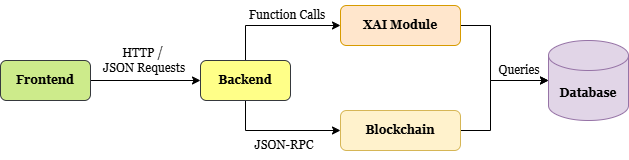
\includegraphics[width=0.95\linewidth]{figures/system_archi_layer.png}
        \label{Four layers of system architecture}
        \caption{4 layers of system architecture}
    \end{figure}

    This framework ensures that every document undergoes AI-driven analysis before any on-chain transaction occurs. If a forged certificate or AI-generated paper is detected, the system rejects the document and never writes it to the blockchain, thereby preventing the immutable recording of fraudulent records.

\section{The Document Processing Pipeline}
    When a document is submitted to the system, it undergoes a multi-step transformation that converts the raw file into machine-analyzable representations. This pipeline is the foundation upon which all subsequent analysis depends.
    \subsection{Multi-Format Text Extraction and Normalization}
    \label{sec:text_extraction_normalization}
        The system supports a broad range of document formats to accommodate real-world usage scenarios in educational and institutional settings. Text extraction is handled by the \texttt{DocumentParser} module, a universal document parser implemented in Node.js. The parser inspects the file extension and delegates to the appropriate extraction library as follows:
        
        \begin{itemize}
            \item \textbf{PDF files} are processed using the \texttt{pdf-parse} library, which reads the binary PDF structure and extracts embedded text layers. If \texttt{pdf-parse} fails (for example, on scanned PDFs without embedded text), the system falls back to \texttt{pdftotext}, a command-line utility from the Poppler project that performs layout-aware text extraction.
        
            \item \textbf{DOCX files} are processed using the \texttt{mammoth} library, which parses the Office Open XML structure and extracts raw text content.
        
            \item \textbf{Plain text formats} (TXT, Markdown, CSV, HTML, TEX) are read directly as UTF-8 encoded strings.
        \end{itemize}
        
        For image-based documents and academic certificates, the system employs Tesseract OCR through the \texttt{tesseract.js} library. Tesseract performs optical character recognition on PNG, JPEG, and WebP images, converting visual text into machine-readable strings. The OCR output includes a confidence score that indicates the reliability of the extraction, which is later factored into the verification decision.
        
         \begin{figure}[H]
        \centering
        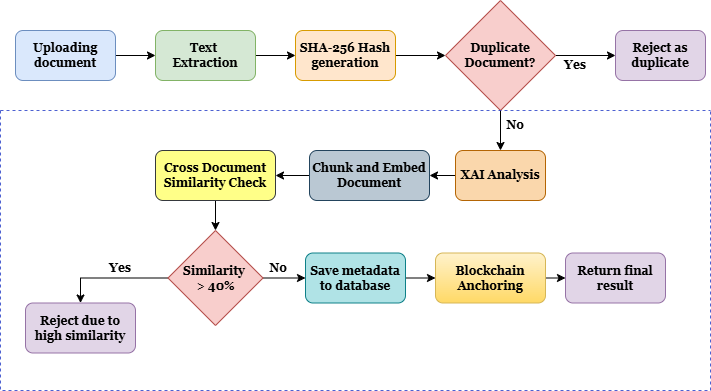
\includegraphics[width=0.95\linewidth]{figures/documet_verification.png}
        \label{Flow of the large-document(article, journal paper) verification}
        \caption{Flow of the large-document(article, journal paper) verification}
        \end{figure}
        After extraction, the text undergoes normalization. The normalization process converts all characters to lowercase, removes non-alphanumeric characters, and collapses multiple whitespace characters into single spaces. This produces a clean, standardized representation that ensures consistent behavior across all downstream analysis modules regardless of the original document format or encoding.

        
    \subsection{Cryptographic Fingerprinting (SHA-256)}
    \label{sec:cryptographic_fingerprint_sha256}
        As soon as a file is uploaded, the system computes a cryptographic hash using the SHA-256 algorithm. This hash serves as the document's digital fingerprint and is central to the entire verification framework. The computation is performed by streaming the file contents through Node.js's built-in \texttt{crypto} module, which produces a 256-bit (64 hexadecimal character) digest.
        
        The choice of SHA-256 is deliberate. First, SHA-256 is a one-way function: given the hash, it is computationally infeasible to reconstruct the original document. Second, it exhibits strong collision resistance, meaning that no two distinct inputs are expected to produce the same output. This property is formally supported by the birthday bound, which places the probability of a collision at approximately \(1 \text{ in } 2^{128}\) for SHA-256, a number so large that accidental collisions are effectively impossible. Third, SHA-256 is deterministic: the same file will always produce the same hash, but even a single-bit change in the input produces a completely different output. This avalanche effect makes SHA-256 ideal for detecting tampering.
        
        The resulting hash is prefixed with \texttt{0x} to maintain compatibility with Ethereum's \texttt{bytes32} data type and serves three purposes in the system. It acts as the primary key for blockchain lookups, enables hash-based deduplication (the system rejects uploads whose hash already exists on-chain or in the database), and provides the immutable link between the off-chain document and its on-chain verification record.
        
        While cryptographic hashing provides certainty about exact document identity, it cannot detect content that has been paraphrased or restructured. The following subsection addresses this limitation.

    \subsection{Vector Embedding and Semantic Indexing}
    \label{sec:vector_embedding}

        Beyond cryptographic hashing, which detects exact byte-level matches, the system requires a mechanism to identify semantic similarity between documents. Two documents may contain the same ideas expressed in different words; a hash comparison would miss this entirely. To address this limitation, the system converts extracted text into dense vector representations using a pre-trained transformer model.
        
        The embedding pipeline operates as follows. First, the document text is split into sentence-level chunks by the \texttt{ChunkingService} module. The chunking process uses a regular expression that matches all text up to and including each sentence-ending punctuation mark (\texttt{.}, \texttt{!}, or \texttt{?}). Each match produces one chunk. Any text remaining after the final punctuation mark is captured as an additional chunk. This approach preserves sentence integrity even when sentences contain abbreviations or decimal numbers.
        
        Before chunking, the service strips the references and bibliography section from academic documents to avoid false similarity matches caused by shared citation entries. The stripping is performed using a multi-strategy approach: the service first searches for explicit reference headers (e.g., ``References'', ``Bibliography'', ``Works Cited'') using a comprehensive regular expression, and if no header is found, it falls back to a citation-density heuristic that detects runs of consecutively formatted citation lines in the latter half of the document.
        
        Each chunk is then passed to the \texttt{EmbeddingService}, which uses the \texttt{Xenova/all-MiniLM-L6-v2} model, a lightweight sentence transformer optimized for semantic similarity tasks. The model produces a 384-dimensional vector for each chunk, where semantically similar texts are mapped to nearby points in the vector space.
        
        These vectors are stored in a PostgreSQL database that has the \texttt{pgvector} extension enabled. When a new document is uploaded, the system queries the database for existing chunks whose cosine distance from the new chunks falls below an embedding similarity threshold (default: 0.25). This allows the system to detect paraphrased plagiarism, where a person has reworded content from another source without copying it verbatim. The embedding-based search produces similarity scores that feed directly into the XAI plagiarism report.


\section{Explainable AI (XAI) Analysis Layer}
\label{sec:Explainable AI}

The XAI Analysis Layer is the core intelligence of the framework. Rather than returning a simple pass/fail verdict, it runs three distinct diagnostic tests and generates human-readable explanations for every finding. By generating human-readable justifications for every finding, the framework closes the accountability gap noted in Chapter 2.5, where users receive opaque binary verdicts from existing verification tools. The three diagnostic modules are described in the following subsections.

    \subsection{Plagiarism and Similarity Auditing}

    The plagiarism detection module operates at two levels to provide comprehensive coverage. At the first level, it performs an internal duplication analysis within the submitted document. The module constructs 8-word n-gram shingles from the normalized text and counts the frequency of each shingle. If the same 8-word sequence appears multiple times, the duplicate shingle count is accumulated and converted into a similarity score. A score exceeding the internal plagiarism threshold of 75\% indicates significant self-repetition within the submitted document and triggers rejection at the XAI module level.
    
    At the second level, the system performs a cross-document similarity search using the vector embeddings described in chapter 3.2.3. Each sentence-level chunk of the newly uploaded document is compared against all existing chunks in the database using cosine similarity. In the production pipeline, the pure embedding similarity is combined with a lexical phrase-overlap score to produce a hybrid similarity metric.
    
    For each uploaded chunk, the system first retrieves embedding-similar candidates from the database. Candidates with sufficiently high embedding similarity then undergo a secondary phrase-overlap analysis, which splits both texts into punctuation-delimited segments and measures the fraction of uploaded segments that appear verbatim in the database text.
    
    The final hybrid score is computed as a weighted average of the embedding similarity and the phrase-overlap score, each contributing 50\%. This two-stage approach combines the semantic generalization of embeddings (which detect paraphrasing) with the precision of exact phrase matching (which reduces false positives from semantically similar but originally authored content).
    
    The system aggregates matches by source document and computes the average hybrid similarity across all chunks. If this average exceeds the cross-document threshold of 40\%, the document is rejected before database storage.
    
    The XAI output for plagiarism detection provides a ``Similarity Map'' that shows the user which sections of the document matched, the similarity percentage for each match, and the source document from which the content appears to have been derived. This transparency allows users to distinguish between legitimate common phrases and genuinely copied content.
    
    \subsection{AI Content Detection}
    \label{sec:ai_content_detection}
    
    The AI content detection module examines the linguistic properties of the extracted text to determine whether it was generated by a large language model or written by a human. The approach is grounded in the Perplexity and Burstiness metrics discussed in Chapter 2.2, which are operationalized through five concrete heuristic indicators:
    
    \begin{enumerate}
        \item \textbf{Lexical Diversity (Perplexity Proxy):} The module calculates the ratio of unique words to total words in the document. Human writing typically exhibits higher lexical diversity (more varied vocabulary), while AI-generated text tends to reuse the same words more frequently. If the lexical diversity falls below 0.34, the module increases the AI probability score by 20 points.
    
        \item \textbf{Sentence Length Variance (Burstiness Proxy):} Human writers naturally produce sentences of varying lengths, some short and punchy, others long and complex. This variation is measured as the statistical variance of sentence lengths across the document. AI-generated text tends to produce sentences of uniform length. If the variance falls below 18, the AI probability score increases by 20 points.
    
        \item \textbf{Repeated Sentence Ratio:} The module normalizes all sentences and counts how many appear more than once. A high ratio of repeated sentences (above 0.14) suggests formulaic generation, adding 25 points to the AI probability score.
    
        \item \textbf{Average Sentence Length:} Excessively long, well-structured sentences (average above 26 words) are more characteristic of AI output, contributing 15 additional points.
    
        \item \textbf{Formal Transition Markers:} The module scans for overuse of formal transition phrases such as ``in conclusion,'' ``moreover,'' ``furthermore,'' ``additionally,'' and ``therefore.'' The presence of these markers adds 10 points, as AI models frequently over-rely on such connectives.
    \end{enumerate}
    
    The composite AI probability score begins at a cautionary baseline of 10 (reflecting the inherent uncertainty in any heuristic classification) and increases as indicators are triggered, up to a theoretical maximum of 100. The five indicator contributions total a maximum of 90 additional points (20 + 20 + 25 + 15 + 10 = 90). If the composite score exceeds the configured threshold of 60\%, the document is flagged as likely AI-generated. The XAI report lists which specific indicators were triggered, allowing users to see exactly which properties of the text raised suspicion. For example, a report might state: ``Low lexical diversity detected; uniform sentence length detected. Language pattern heuristic suggests likely AI-generated content.''


    \subsection{Certificate Forgery Isolation}
    \label{sec:Cert_forgery_isolation}
    
    For documents classified as certificates, the system runs a specialized forgery detection module. This module analyzes the structural elements that legitimate certificates are expected to contain. The detection proceeds by checking for four key structural signals using regular expression pattern matching against the OCR-extracted text:
    
    \begin{enumerate}
        \item \textbf{Date Presence:} The module searches for date patterns in various formats (DD/MM/YYYY, Month DD, YYYY, etc.) using a comprehensive set of regular expressions. Legitimate certificates almost always contain an issuance date.
    
        \item \textbf{Certificate Identifier:} The module looks for registration numbers, serial numbers, roll numbers, or other identifier patterns that typically follow keywords such as ``Certificate No.'' or ``Registration No.''
    
        \item \textbf{Issuer Information:} The module checks for institutional keywords such as ``University,'' ``Institute,'' ``Board,'' ``Authority,'' ``Department,'' or ``Ministry'' that indicate the document was issued by a recognized body.
    
        \item \textbf{Signature Block:} The module searches for keywords associated with authorization, such as ``Signature,'' ``Signed,'' ``Registrar,'' ``Controller,'' ``Principal,'' or ``Dean.''
    \end{enumerate}
    
    Each missing signal contributes 25 points to a forgery risk score. If two or more signals are absent (score $\geq 50$), the certificate is flagged as potentially forged. The XAI explanation lists which signals were missing, providing the user with a clear and understandable justification. For instance: ``Certificate consistency heuristic flagged missing signal(s): date, signature\_block.''

    \subsection{Result Combination and Confidence Scoring}
    \label{sec:result_comb_score}
    
    After the three diagnostic tests complete, the \texttt{RealXAIAnalyzer} module combines their outputs into a unified verification result. The combination logic works as follows:
    
    The system starts with a base confidence score of 100. If the plagiarism check detects significant similarity, the score is reduced by 40 points and the document status is set to ``rejected.'' If AI-generated content is detected, the score is further reduced by 35 points. If certificate forgery is detected, the confidence score is set to 0, as this represents the most critical type of fraud.
    
    For documents that pass all checks, the confidence score is adjusted proportionally based on the individual sub-scores (e.g., a moderate AI probability that remains below the threshold will still cause a small deduction).
    
    The final output includes the overall status (verified or rejected), the confidence score, a timestamp, detailed results from each diagnostic module, a list of rejection reasons (if any), and a human-readable explanation object that summarizes the findings in plain language.


\section{Certificate Verification Methodology}
\label{sec:certificate_verification_method}

    The system implements a dedicated certificate verification workflow that is distinct from the large-document verification pipeline. This workflow is designed specifically for small-format credentials such as academic certificates, diplomas, and professional licenses. The verification proceeds through the following stages.

      \begin{figure}[H]
        \centering
        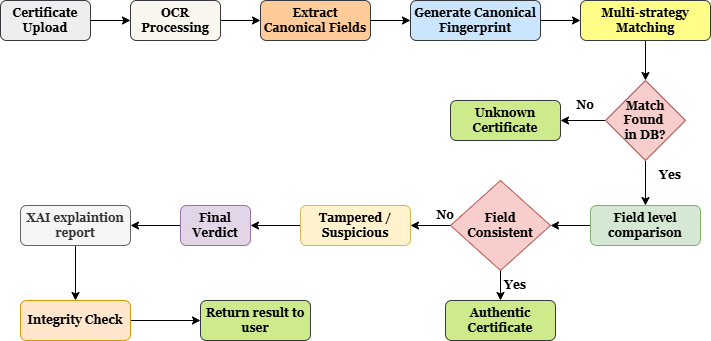
\includegraphics[width=0.95\linewidth]{figures/certificate_verification.png}
        \label{The certificate verification workflow}
        \caption{The certificate verification workflow}
        \end{figure}    
    
    \subsection{OCR and Field Extraction}
    \label{sec:ocr_field_extraction}
    
        When a certificate is uploaded for verification, the system first performs OCR using Tesseract to extract all visible text from the document image. The extracted text is then passed to the \texttt{certificate-field-extractor} module, which uses a library of specialized regular expression patterns to identify five canonical fields:
        
        \begin{enumerate}
            \item \textbf{Recipient Name:} Detected by patterns such as ``awarded to [Name],'' ``presented to [Name],'' or ``this is to certify that [Name].''
        
            \item \textbf{Course or Title:} Detected by patterns such as ``has completed the course [Title]'' or ``for the degree of [Title].''
        
            \item \textbf{Issue Date:} Detected by multiple date format patterns including ISO format, DD/MM/YYYY, and natural language dates.
        
            \item \textbf{Certificate Serial:} Detected by patterns following keywords such as ``Certificate No'' or ``Registration No.''
        
            \item \textbf{Issuer Name:} Detected by institutional keywords and patterns such as ``issued by [Institution].''
        \end{enumerate}
        
        Each extracted field includes a confidence score indicating the reliability of the extraction. These five fields form the canonical representation of the certificate.
        
    \subsection{Canonical Fingerprinting}
    \label{sec:fingerprint}
    
        The extracted canonical fields are used to compute a canonical fingerprint. This fingerprint is generated by sorting the field names alphabetically, normalizing each field value (lowercasing, removing special characters, collapsing whitespace), and computing the SHA-256 hash of the resulting JSON string.
        
        This canonical fingerprint provides a content-based identifier that remains stable even if the certificate is re-scanned at different resolutions or with minor visual variations, as long as the textual content remains the same.
    
    \subsection{Multi-Strategy Record Matching}
    \label{sec:multi_strategy_matching}

        To find the corresponding registered certificate, the system employs a cascading multi-strategy matching approach. The system attempts to match the uploaded certificate against existing records using the following strategies, in order of specificity:
        
        \begin{enumerate}
            \item \textbf{Certificate ID Match:} If the user provides a known certificate ID, the system looks it up directly.
        
            \item \textbf{File Hash Match:} The SHA-256 hash of the uploaded file is compared against stored hashes. A match indicates a byte-for-byte identical copy of the original registered certificate.
        
            \item \textbf{Serial Number Match:} The extracted or user-provided serial number is searched against the certificate database.
        
            \item \textbf{Canonical Fingerprint Match:} The computed canonical fingerprint is compared against the fingerprints of all registered certificates.
        \end{enumerate}
        
        The system proceeds through these strategies sequentially and stops at the first successful match. If no match is found through any strategy, the system reports the certificate as ``unknown'' (not registered) or ``not a certificate'' (if the forgery check determined that the document lacks essential certificate characteristics).
        
        \subsection{Field-Level Comparison and Verdict}
        \label{sec:comparison_verdict}
        
        When a matching record is found, the system performs a field-by-field comparison between the canonical fields extracted from the uploaded certificate and those stored in the database during issuance. Each field comparison produces one of the following statuses:
        
        \begin{itemize}
            \item \textbf{Exact:} The normalized values are identical.
        
            \item \textbf{Whitespace Only:} The values differ only in whitespace.
        
            \item \textbf{Date Format Match:} The dates represent the same calendar date in different formats.
        
            \item \textbf{Fuzzy Full:} All significant words from the expected value appear in the found value.
        
            \item \textbf{Fuzzy Partial:} At least 60\% of significant words overlap between the two values.
        
            \item \textbf{Mismatch:} The values differ substantially.
        \end{itemize}
        
        Based on the comparison results, the system assigns one of five verdicts: \textbf{Authentic} (file hash matches or all key fields match exactly), \textbf{Tampered} (one or more fields differ from the registered record), \textbf{Revoked} (the certificate has been explicitly revoked by the issuing organization), \textbf{Suspicious} (partial matches that do not meet the threshold for authenticity), or \textbf{Unknown} (no matching record found).
        
        The XAI analysis for each verdict includes structured reasons, evidence items (including the specific fields that differed and their expected vs.\ found values), and actionable recommendations. For example, a ``tampered'' verdict might include: ``The recipient name on the document does not match the registered record. This is the most common sign of certificate forgery.''

\section{The Blockchain Trust Layer}
\label{sec:blockchain_layer}
    Once the XAI analysis is complete and the document passes pre-validation, the verification results are anchored to the blockchain through the \texttt{DocumentRegistry} smart contract. This section describes the smart contract design and the anchoring process.
    \subsection{Smart Contract Design}
    \label{sec:smart_contract}
        The \texttt{DocumentRegistry} contract is written in Solidity 0.8.24 and deployed on a Hardhat-managed Ethereum-compatible local network (chain ID 1337). The contract defines a \texttt{Document} struct that stores the following fields for each registered document:
        
        \begin{itemize}
            \item \texttt{documentHash} (\texttt{bytes32}): The SHA-256 hash of the document file.
        
            \item \texttt{documentName} (\texttt{string}): A human-readable identifier for the document.
        
            \item \texttt{uploader} (\texttt{address}): The Ethereum address that registered the document.
        
            \item \texttt{timestamp} (\texttt{uint256}): The Unix timestamp of registration.
        
            \item \texttt{isVerified} (\texttt{bool}): The verification status.
        
            \item \texttt{xaiAnalysis} (\texttt{string}): A JSON-encoded summary of the XAI analysis results.
        
            \item \texttt{verificationStatus} (\texttt{string}): A descriptive status string (e.g., ``pending,'' ``verified,'' ``rejected'').
        
            \item \texttt{confidenceScore} (\texttt{uint256}): The XAI confidence score on a scale of 0--100.
        \end{itemize}
        
        The contract exposes six primary functions: \texttt{registerDocument} for creating new entries, \texttt{addXAIAnalysis} for attaching analysis results, \texttt{verifyDocument} for updating the verification status, \texttt{getDocument} for retrieving full document details, \texttt{documentExists} for existence checks, and \texttt{getVerificationStatus} for lightweight status queries.
        
        \subsection{Three-Step Anchoring Process}
        \label{sec:three_step_anchoring}
        
        When the backend server registers a document on the blockchain, it executes three sequential transactions through the \texttt{BlockchainConnector} module:
        
        \begin{enumerate}
            \item \textbf{Registration:} The \texttt{registerDocument} function is called with the document hash and name. The contract checks that the hash does not already exist (preventing duplicate registrations) and records the document with a ``pending'' status.
        
            \item \textbf{XAI Analysis Attachment:} The \texttt{addXAIAnalysis} function is called with a JSON summary of the XAI results. To minimize gas costs, the system stores only a compact summary on-chain (status, similarity score, AI probability, and match count) rather than the full analysis report, which is persisted in the PostgreSQL database.
        
            \item \textbf{Verification:} The \texttt{verifyDocument} function is called with the final verification status and confidence score. This marks the document as verified on the blockchain, creating an immutable record that can be independently verified by any third party.
        \end{enumerate}
        
        Each transaction emits a Solidity event (\texttt{DocumentRegistered}, \texttt{XAIAnalysisAdded}, \texttt{DocumentVerified}) that provides an auditable log of all state changes. The gas consumption for each transaction is tracked and reported, which enables the performance analysis discussed in Chapter 5.

        \subsection{Verification and Re-Anchoring}
        \label{sec:verification_reanchroing}

            When a third party wants to verify a document, the system re-computes the SHA-256 hash of the submitted file and queries the blockchain through the \texttt{documentExists} and \texttt{getDocument} functions. If the hash exists on-chain and the stored status is ``verified,'' the document is confirmed as authentic.
            
            If the hash is not found on the current blockchain instance (for example, because the local Hardhat node was restarted), the system can automatically re-anchor the document by re-executing the three-step registration process, provided that the document record still exists in the PostgreSQL database. This re-anchoring mechanism ensures continuity of verification even across blockchain restarts.
            
            \section{Neon PostgreSQL (Cloud Database)}
            \label{sec:Neon_database}
            
            The system uses Neon, a serverless PostgreSQL platform, as its primary relational storage engine. PostgreSQL was selected over alternative databases for three reasons: its support for the \texttt{pgvector} extension (which enables native vector similarity search), its ACID compliance (which guarantees data consistency), and its ability to store binary data (which allows certificate files to be stored directly in the database).
            
            The database manages the following categories of data:
            
            \begin{enumerate}
                \item \textbf{Document Records:} Each uploaded document is stored with its filename, SHA-256 hash, upload timestamp, and a JSON metadata column that holds the XAI analysis results, blockchain transaction data, uploader information, and document type classification.
            
                \item \textbf{Sentence-Level Chunks:} The text of each document is split into sentence-level chunks, each stored with its content, chunk index, SHA-256 content hash, token count, a simple word-frequency embedding (a 100-dimensional JSON array derived from normalized word counts within the chunk, used as a lightweight fallback for basic text fingerprinting), and a dense transformer embedding (384-dimensional, stored as a \texttt{vector(384)} column via \texttt{pgvector}, used for semantic similarity search as described in chapter 3.2.3.
            
                \item \textbf{Certificate Records:} Issued certificates are stored with their canonical fields (recipient name, course title, issue date, serial number, issuer name), the canonical fingerprint, the file hash, the original document binary, OCR text, blockchain anchoring data, and status information (active, revoked).
            
                \item \textbf{Organization Records:} Issuing organizations are registered with API key hashes, contact information, and activation status.
            \end{enumerate}
            
            The \texttt{pgvector} extension enables the system to perform cosine similarity searches directly in SQL, using the \texttt{<=>} operator to compare embedding vectors. This eliminates the need for a separate vector database and simplifies the deployment architecture.
        
        \section{User Interaction and Interface}
        \label{sec:user_interface}

            The system presents verification results through a web-based dashboard built with Next.js. The interface is designed to make the complex multi-layered analysis accessible to non-technical users. The verification result display includes the following components:
            
            \begin{enumerate}
                \item \textbf{The Verdict:} A prominent visual indicator showing the overall verification status (Verified, Suspicious, Tampered, Revoked, or Unknown) along with the confidence score.
            
                \item \textbf{The XAI Explanation:} A structured breakdown showing exactly how the AI arrived at its decision. For document verification, this includes the plagiarism similarity score with matched sections, the AI detection probability with triggered indicators, and (for certificates) the forgery risk assessment with missing structural signals. For certificate verification, this includes the field-by-field comparison table showing expected versus found values for each canonical field.
            
                \item \textbf{Blockchain Receipt:} A verifiable link to the on-chain transaction, including the transaction hash, block number, contract address, and timestamp. This provides an independent, tamper-proof record that the verification occurred and what the result was.
            
                \item \textbf{Actionable Recommendations:} Based on the analysis findings, the system provides specific guidance. For example, if a certificate's recipient name does not match the registered record, the recommendation explicitly states that this is the most common sign of certificate forgery and advises manual review.
            \end{enumerate}
        
        





%     This chapter provides a comprehensive technical breakdown of the Integrated Document Verification Platform. The methodology is designed to create a seamless journey from the moment a user uploads a document to the final generation of a transparent and blockchain-anchored verification report.
    
% \section{Overall System Architecture}
%     The framework is built on a Modular Hybrid Architecture  meaning it divides tasks between three specialized engines. Those are the Web Orchestrator, the Blockchain Trust Layer and the Explainable AI (XAI) Analysis Layer.
%     \\
%     Think of the system as a high-security airport check-point:
%     \\
% \begin{enumerate}
%     \item \textbf{The Orchestrator (The Guard): }Receives the document and checks for basic requirements.
%     \item \textbf{The XAI Module (The Specialist):} Inspects the document deeply for "micro forgeries" or AI generated text and explains the red flags.
%     \item \textbf{The Blockchain (The Ledger):} Permanently records the final status so it can never be changed.
%     \item \textbf{The Data \& Trust Tier (Neon DB \& Blockchain):} A dual layered storage approach where metadata and vector embeddings are stored in the cloud (Neon), while cryptographic proofs are anchored to the blockchain. 


% \end{enumerate}

%     \begin{figure}[H]
%             \centering
%             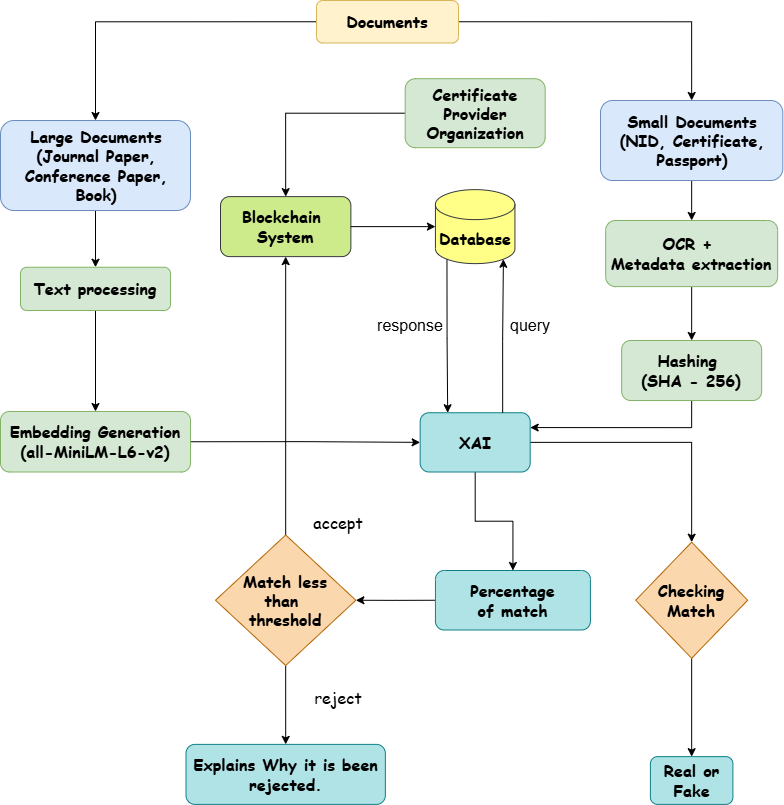
\includegraphics[width=0.95\linewidth]{figures/system_archi.png}
%             \label{Article or Journal paper verification UI}
%             \caption{System Architecture}
%         \end{figure}
 
% \section{The Document Processing Pipeline}
%     When a document is submitted, it undergoes a four-step transformation:

%     \subsection{Multi-Format Text Extraction \& Normalization }\label{ss:transformer}
%     Since our tool has a robust extraction layer, it allows for the handling of many document types. This feature is achieved by leveraging such modules as PyPDF2, python-docx and Tesseract OCR which are used for retrieving the text content and formatting information of over 15 file formats. This stage is essential since at this point the data is cleaned up, making the analysis more consistent. At this stage unimportant data is eliminated, and the AI receives necessary insights into the essence of the text and its structural properties. 
    
%     \subsection{ Cryptographic Fingerprinting (SHA-256) }\label{ss:transformer}
% \begin{enumerate}
%         \item As soon as a file is uploaded to the system, a Digital Fingerprint is produced based on the SHA-256 approach.
%         \item At this stage, a hash function creates a digital fingerprint consisting of 64 characters.
%         \item At first sight, the primary function of the code is to uniquely identify the file. Due to the one-way nature of SHA-256 algorithm even slightest changes made to the document lead to generation of an entirely different code.
%     \end{enumerate}

%      \subsection{Vector Embedding }\label{ss:transformer}

%      The system does not just look for keywords it uses Natural Language Processing to turn text into mathematical codes. These codes show what the text means, not just the words. The system stores these codes in PostgreSQL. Can search for similar codes. This helps the system find plagiarism even when someone has changed the words but kept the ideas. The Document Processing Pipeline and the Vector Embedding process are parts of the system. The Document Processing Pipeline is used to process the documents and the Vector Embedding is used to find documents. 
% \section{Explainable AI (XAI) Analysis Layer}\label{sec:prop_archi}
% This is the "intelligence" of the system. Instead of a simple pass/fail, it runs three distinct diagnostic tests:
%      \subsection{AI Content Detection }\label{ss:transformer}
%      Using the \texttt{ai\_content\_detector.py} module, the system calculates the "Perplexity" and "Burstiness" of the text. Human writing is naturally inconsistent (high burstiness), while AI writing tends to be very uniform. The XAI component highlights these uniform sections to show the user exactly which paragraphs look "machine-made."
%      \subsection{Certificate Forgery Isolation}\label{ss:transformer}
%      The system analyzes the layout of academic certificates. It looks for "Structural Anomalies"—such as inconsistent font metadata or manipulated background layers—that are common in forged diplomas but absent in originals.
%      \subsection{Plagiarism \& Similarity Auditing}\label{ss:transformer}
%      By querying the vector database, the system identifies if large portions of the document have been copied from elsewhere. The XAI interface provides a "Similarity Map," showing the source and the percentage of matched content.
%      \subsection{ The Blockchain Trust Layer
%     }\label{ss:transformer}
%     Once the AI completes its audit, the results are sent to the Ethereum-based Smart Contract (DocumentRegistry.sol).
%     \begin{enumerate}
%         \item \textbf{Immutable Anchoring:} The system writes the SHA-256 hash, the XAI "Trust Score," and the timestamp into a permanent block. Once confirmed, this data cannot be modified by any administrator or hacker.
%         \item \textbf{Decentralized Access Control:} The smart contract defines roles (e.g., "Issuer," "Verifier," "Admin"). Only authorized institutions can issue a "Verified" status, but anyone with the original file can query the contract to confirm its authenticity.
%         \item \textbf{The Consensus Check:} When a third party verifies a document, the system re-calculates the hash in real-time. It then queries the blockchain: "Does this new hash exist in the registry?" If the hashes match, the document is authentic.

%     \end{enumerate}
%     \section{Neon PostgreSQL (Cloud Database)}
%     This architecture relies on Neon, a PostgreSQL serverless environment, as the main relational storage engine. The database manages:
%     \begin{enumerate}
%         \item \textbf{User Profiles and Meta Information:} Holds user accounts, institution information, and document metadata.
%         \item \textbf{Vector Embeddings:} With pgvector extension support, the solution will use mathematically encoded document texts. It provides fast searching capabilities that detect semantic similarities (plagiarism) that cannot be done directly through a blockchain.
%         \item \textbf{System Logs:} Holds transaction history and XAI report summaries for dashboard generation.
%     \end{enumerate}


% \section{User Interaction and Interface}
% Finally, the system ends with displaying the verification results in a Verification Dashboard. The following points outline this simple yet effective UI design:
% \begin{enumerate}
%     \item \textbf{The Verdict:} A verdict is given(Verified/Suspicious).
%     \item \textbf{The "Why" (XAI Output):} A visual representation of how AI came up with such a decision (for example, "90% probability of an AI-generated text in Section 2").
%     \item \textbf{Blockchain Receipt:} A link to the transaction on the blockchain network to ensure the result is official and irrefutable.

% \end{enumerate}


% \section{Chapter Summary}
% In Chapter 3, we reviewed in detail the workflow of the hybrid model in action. Starting from uploading the document to the system all the way to the cryptographic hash generation and subsequent vectorization, moving further on to the analysis conducted by the AI, we ended up exploring the role of Blockchain technology in securing these conclusions.